\section{W10: Agile Frameworks}

\textbf{SAFe Agile}: Scaled Agile Framework.
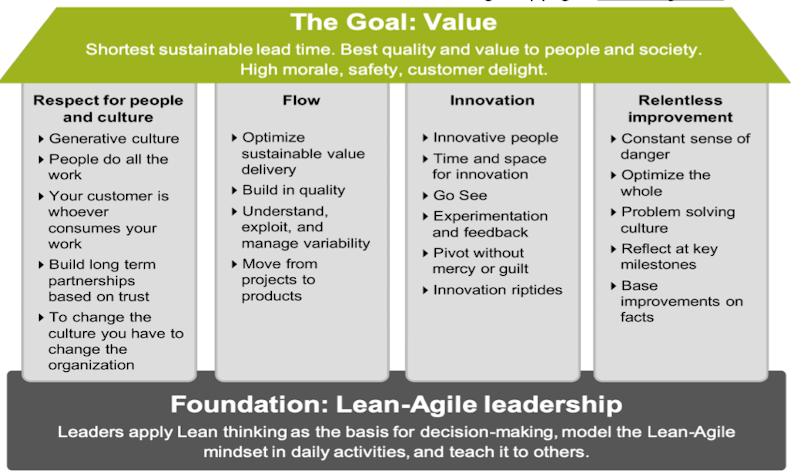
\includegraphics[width=\linewidth]{figs/SCR-20240606-podj.png}
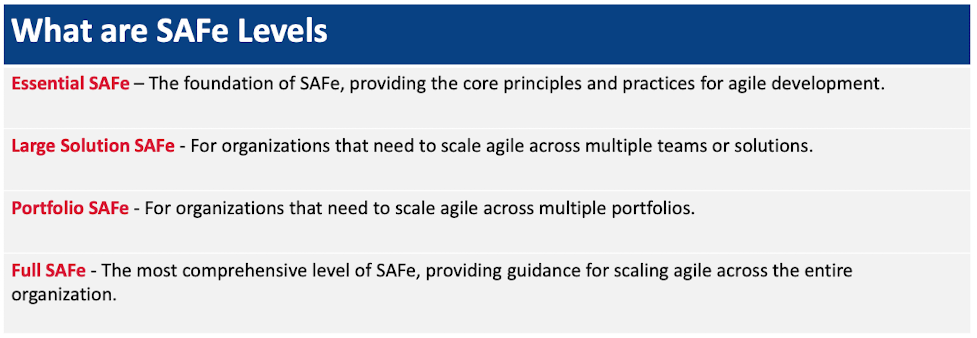
\includegraphics[width=\linewidth]{figs/SCR-20240606-prfh.png}

\textbf{Large Scale Scrum (LeSS).}
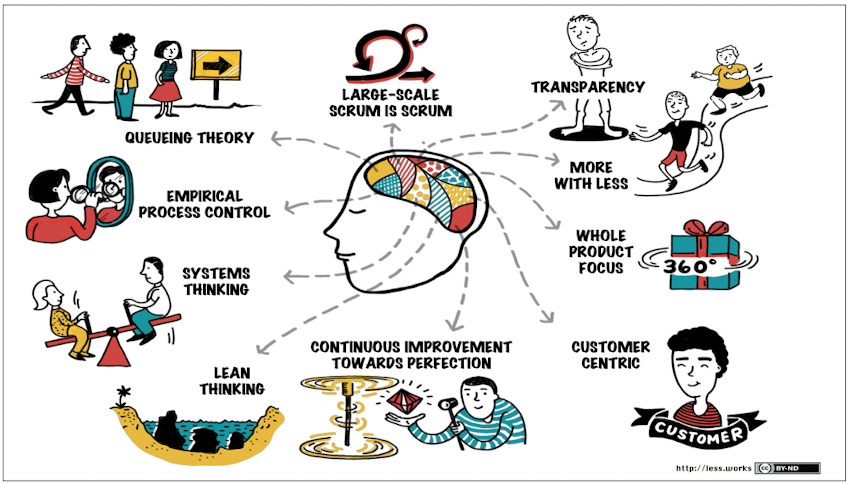
\includegraphics[width=\linewidth]{figs/SCR-20240606-prmd.png}
In standard Scrum, each team conducts its own retrospective at the end of the sprint. In LeSS, there is an additional "Overall Retrospective" that involves members from multiple teams.

In Scrum, there is only one sprint planning meeting. In LeSS, there are two. Sprint 1 focuses on determining what work will be selected from the product backlog, and Sprint 2 focuses on how the work will be done.

LeSS is a scaled-up version of one-team Scrum. It has a single product backlog, one DoD, one Potentially Shippable Product Increment at the end of each Sprint, one Product Owner, many complete, cross-functional teams, one Sprint.

\textbf{Scrum@Scale.}

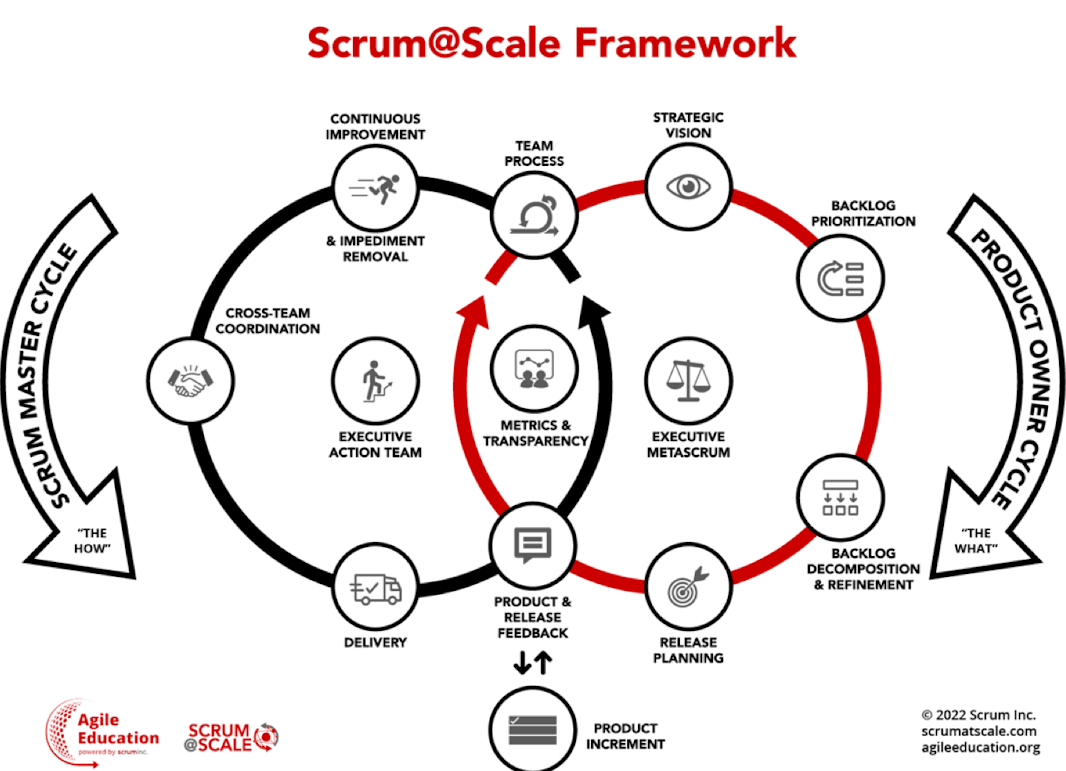
\includegraphics[width=\linewidth]{figs/SCR-20240606-swrt.png}
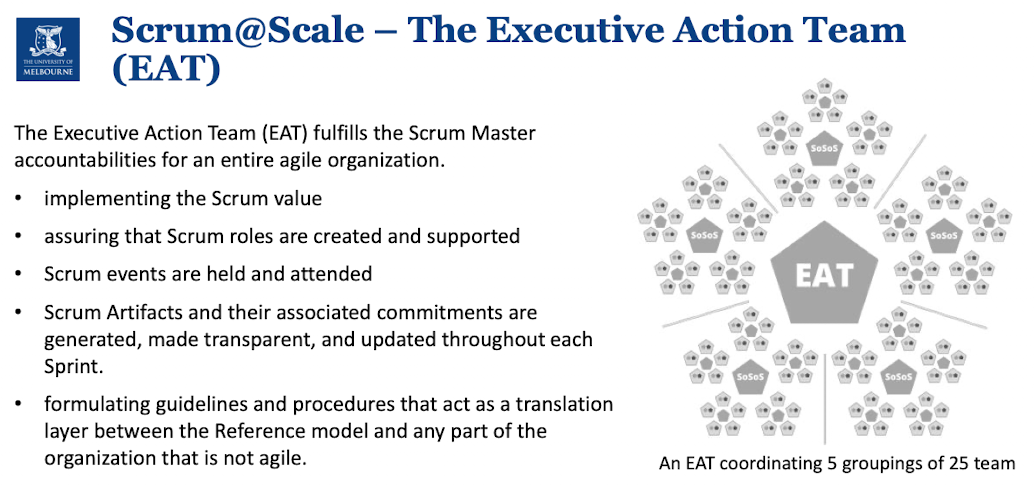
\includegraphics[width=\linewidth]{figs/SCR-20240606-szho.png}

\textbf{DevOps.}

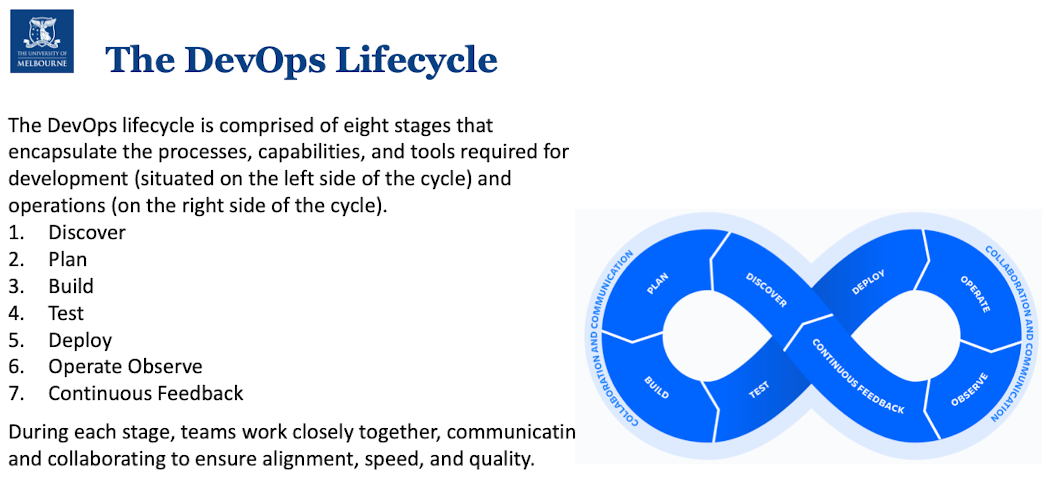
\includegraphics[width=\linewidth]{figs/SCR-20240606-taig.png}

\textbf{Lean Software Development.}

7 principles: (1) eliminate waste, (2) build in quality (using TDD or Pair Programming), (3) amplify learning (knowledge gained must be shared), (4) delay commitment as long as possible, (5) deliver fast, (6) respect people (encourage proactive feedback and constant feedback), (7) optimise the whole (make the lean value stream as efficient as possible).